\section{Failure Handling}

A transaction constitutes an indivisible transformation from an initial state to a final state. 
The potential outcomes of a transaction include: \texttt{commit}, \texttt{rollback}, or \texttt{fault}.

In the event of a failure occurring between commit and the flushing of buffers to secondary storage, the reliability manager ensures the rolling forward of transactions and the subsequent flushing of buffers to disk. 
If a failure occurs before commit, the reliability manager rolls back the transactions, discarding any modifications made to the buffers.
\begin{example}
    Assuming the DBMS initiates at time $T_0$ and experiences a failure at $T_f$, with data for transactions $T_2,T_3$ committed and permanently stored, transactions $T_1,T_6$ need to be undone.
    In the absence of information on whether modified pages have been flushed, the reliability manager must redo $T_4$ and $T_5$.
    \begin{figure}[H]
        \centering
        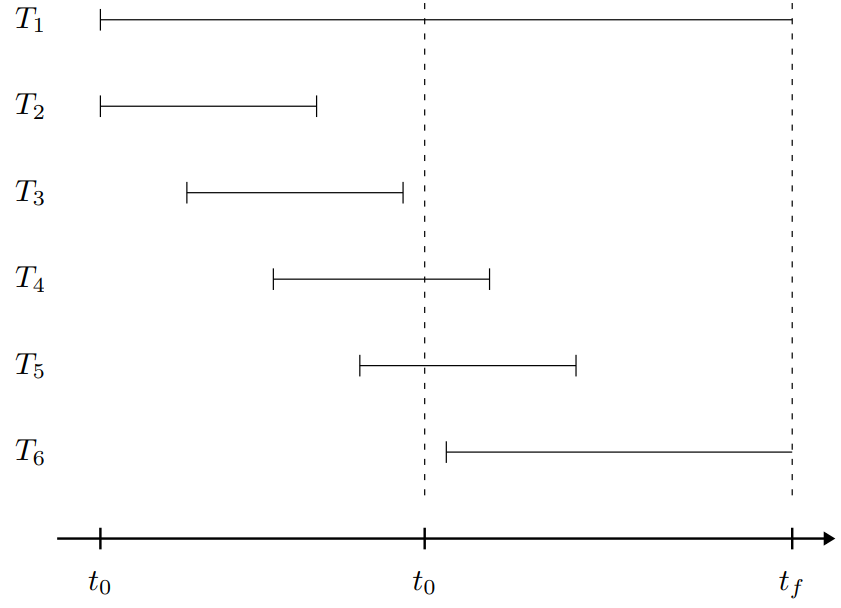
\includegraphics[width=0.5\linewidth]{images/tar.png}
        \caption{Architecture of a DBMS}
    \end{figure}
\end{example}

\subsection{Transaction Log}
The transaction log is a sequentially written file containing records that describe the actions undertaken by various transactions. 
It extends up to the current instant.
\begin{figure}[H]
    \centering
    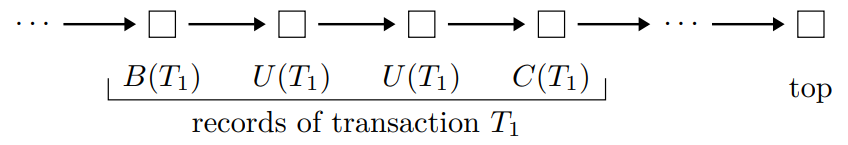
\includegraphics[width=0.5\linewidth]{images/tl}
    \caption{Architecture of a DBMS}
\end{figure}
The log, recorded in stable memory, takes the form of state transitions detailing the actions carried out by transactions.
For an update $U$ operation transforming object $O$ from value $v_1$ to $v_2$, the log contains:
\begin{itemize}
    \item \texttt{before-state(U)} = $v_1$
    \item \texttt{after-state(U)} = $v_2$
\end{itemize}
Logging \texttt{INSERT} and \texttt{DELETE} operations is the same as logging \texttt{UPDATE} operations, but:
\begin{itemize}
    \item \texttt{INSERT} log record does not have a \texttt{before-state}.
    \item \texttt{DELETE} log record does not have an \texttt{after-state}.
\end{itemize}
\begin{example}
    Consider a transaction $T_1$ updating object $O$ from value $O_1$ to $O_2$.
    To rollback the transaction or rectify a pre-commit failure, the log is utilized to recover the prior state:
    \[\texttt{undo }T_1:O=O_1\]
    To address a post-commit failure, the log is used to recover the new state:
    \[\texttt{redo }T_1:O=O_2\]
\end{example}
The idempotence property applies to \texttt{undo} and \texttt{redo}: 
\begin{itemize}
    \item \texttt{undo}(T) = \texttt{undo}(\texttt{undo(T)}).
    \item \texttt{redo}(T) = \texttt{redo}(\texttt{redo(T)}).
\end{itemize}
Idempotence is crucial for the reliability manager, as it may need to apply these operations multiple times. 
For instance, if a failure occurs after the commit of $T_1$ and the log is not flushed, the reliability manager applies \texttt{redo} to $T_1$ and then $T_2$.
This property ensures repeated application without altering the database state.

\paragraph*{Log types}
The logs concerning transactional commands are: 
\begin{itemize}
    \item \texttt{B(T)}: begin transaction \texttt{T}.
    \item \texttt{C(T)}: commit transaction \texttt{T}.
    \item \texttt{A(T)}: abort transaction \texttt{T}.
\end{itemize}
The logs concerning \texttt{UPDATE}, \texttt{DELETE} and \texttt{INSERT} operations are:
\begin{itemize}
    \item \texttt{U(T, O, v\_1, v\_2)}: update object \texttt{O} from value \texttt{v\_1} to value \texttt{v\_2} in transaction \texttt{T}.
    \item \texttt{D(T, O, v)}: delete object \texttt{O} with value \texttt{v} in transaction \texttt{T}.
    \item \texttt{I(T, O, v)}: insert object \texttt{O} with value \texttt{v} in transaction \texttt{T}.
\end{itemize}

\paragraph{Transactional rules}
Log management must ensure that transactions implement \texttt{write} operations reliably. 
To achieve this, the reliability manager adheres to the following rules:
\begin{enumerate}
  \item A commit log record must be written synchronously (with a force operation).
  \item The before-state must be written in the log before executing the corresponding operation on the database (write-ahead logging).
  \item The after-state must be written in the log before executing the commit (commit rule).
\end{enumerate}
The second rule ensures that actions can be undone in case of failure, while the third rule ensures that actions can be redone in case of failure.

\subsection{Failures types}
There are three types of failures:
\begin{itemize}
    \item Soft failure: loss of part or all of the main memory and requires a warm restart. 
        To replay the transactions it is possible to exploit the log. 
    \item Hard failure: failure or loss of part or all of the secondary memory devices and requires a cold restart. 
        To replay the transactions it is possible to exploit the dump. 
    \item Disaster: loss of stable memory (of the log and the dump).
\end{itemize}

\subsection{Checkpointing}
Checkpoints serve to minimize the amount of work needed in case of failure by capturing snapshots of the database and log at a specific time.
Periodically, the Reliability Manager initiates checkpoints, where committed transactions flush their data from the buffer to the disk, and all active transactions are recorded in the log.
A straightforward checkpointing strategy involves the following steps:
\begin{enumerate}
    \item Acceptance of all transactions that have committed their work.
    \item Suspension of all abort requests.
    \item Forceful transfer of all dirty buffer pages modified by committed transactions to mass storage.
    \item Recording the identifiers of transactions still in progress in the checkpoint log record; no new transaction can start while this record is being written.
    \item Resumption of the acceptance of operations.
\end{enumerate}
This ensures that all data related to committed transactions resides on mass storage, while transactions still in progress are listed in the checkpoint log record (in stable memory).

\paragraph*{Dump}
A dump is a comprehensive backup of the database at a specific time. 
Dumps are typically created during periods of low database activity, such as at night or over the weekend. 
The availability of the dump is recorded in the log, while the dump's content itself is stored in stable memory.

\subsection{Database restarting}

\paragraph*{Warm restart}
The warm restart is performed according to the following steps:
The warm restart involves the following steps:
\begin{enumerate}
    \item Finding the most recent checkpoint.
    \item Building the \texttt{UNDO} and \texttt{REDO} sets:
        \begin{lstlisting}[style=Java]
UNDO := active transactions in the checkpoint
REDO := {}
for log records from the checkpoint to the top of the log do:
    if B(T_i) then
        UNDO := UNDO $\cup$ {T_i} // started, maybe undone
    else if C(T_i) then
        UNDO := UNDO $\setminus$ {T_i}
        REDO := REDO $\cup$ {T_i} // ended, to redo
    end if
end for
        \end{lstlisting}
    \item Undoing the transactions in the \texttt{UNDO} set by applying the \texttt{UNDO} operations in reverse order.
    \item Redoing the transactions in the \texttt{REDO} set by applying the \texttt{REDO} operations.
\end{enumerate}

\paragraph*{Cold restart}
The cold restart involves the following steps:
\begin{enumerate}
\item Restoring data starting from the last backup (dump).
\item Replaying operations recorded into the log before the failure time.
\item Restoring data on disk to the state existing at the failure time.
\item Performing a warm restart.
\end{enumerate}
During the cold restart, uncertain transactions are undone.